\chapter{Diseño del Sistema}

\section{Selección de Componentes}

El sistema se compone de los siguientes elementos principales:

\begin{table}[h]
\centering
\caption{Componentes del Sistema}
\label{tab:componentes}
\begin{tabular}{llll}
\toprule
\textbf{Componente} & \textbf{Modelo} & \textbf{Cantidad} & \textbf{Propósito} \\
\midrule
ODrive v3.6 Oficial & v3.6 & 1 & Control 1 motor (Hip 1) \\
Makerbase ODrive & M1 M22015 & 1 & Control 2 motores (Hip 2 + Knee) \\
Motor BLDC & D5065 270KV & 3 & Actuación (por pierna) \\
Encoder & AS5600 & 3 & Posición articular (por pierna) \\
Multiplexor I2C & TCA9548A & 1 & Lectura de encoders \\
Controlador Principal & Raspberry Pi & 1 & Control de alto nivel \\
\bottomrule
\end{tabular}
\end{table}

\section{Configuración de la Pierna (3-DOF, Sin Tobillo)}

La pierna robótica utiliza un pie de tipo bola (ball foot) y no tiene articulación de tobillo. La configuración de las articulaciones es:

\begin{table}[h]
\centering
\caption{Configuración de Articulaciones}
\label{tab:articulaciones}
\begin{tabular}{lllllll}
\toprule
\textbf{Articulación} & \textbf{Eje Rotación} & \textbf{ODrive} & \textbf{Eje ODrive} & \textbf{Offset Z (m)} & \textbf{Rango (rad)} & \textbf{Reducción} \\
\midrule
Hip 1 (Abd/Add) & X & Oficial & 0 & 0 & $\pm$0.79 & 16:1 \\
Hip 2 (Flex/Ext) & Y & Makerbase & 0 & -0.04 & $\pm$0.52 & 16:1 \\
Knee (Flex/Ext) & Y & Makerbase & 1 & -0.39 & -1.57 a 0 & 16:1 \\
Pie de Bola & - & - & - & -0.74 & - & - \\
\bottomrule
\end{tabular}
\end{table}

Sistema de coordenadas (pierna derecha): +X = Frente, +Y = Izquierda, +Z = Arriba. Pierna extendida apunta en -Z.

Longitudes de eslabones: $L_1 = 0.04$m (Hip1→Hip2), $L_2 = 0.35$m (Hip2→Knee), $L_3 = 0.35$m (Knee→Foot). Total cadera-pie: 0.74m.

\section{Arquitectura del Sistema}

\begin{figure}[h]
\centering
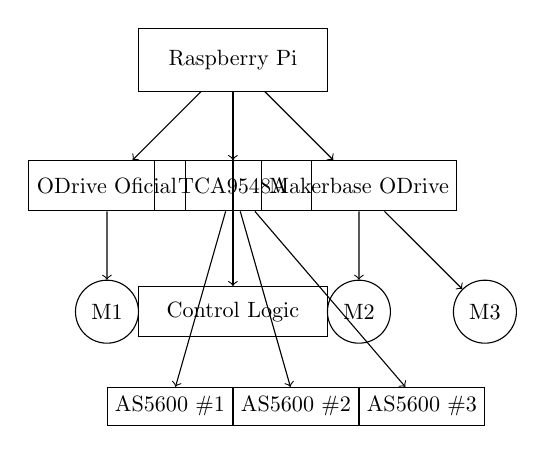
\begin{tikzpicture}[scale=0.8, every node/.style={transform shape}]
% Raspberry Pi
\node[draw, rectangle, minimum width=3cm, minimum height=1cm] (pi) at (0,0) {Raspberry Pi};
% ODrives
\node[draw, rectangle, minimum width=2.5cm, minimum height=0.8cm] (off) at (-2,-2) {ODrive Oficial};
\node[draw, rectangle, minimum width=2.5cm, minimum height=0.8cm] (mk) at (2,-2) {Makerbase ODrive};
% I2C Mux
\node[draw, rectangle, minimum width=2.5cm, minimum height=0.8cm] (mux) at (0,-2) {TCA9548A};
% Control Logic
\node[draw, rectangle, minimum width=3cm, minimum height=0.8cm] (ctrl) at (0,-4) {Control Logic};

% Connections
\draw[->] (pi) -- (off);
\draw[->] (pi) -- (mk);
\draw[->] (pi) -- (mux);
\draw[->] (pi) -- (ctrl);

% Motors
\node[draw, circle, minimum size=1cm] (m1) at (-2,-4) {M1};
\node[draw, circle, minimum size=1cm] (m2) at (2,-4) {M2};
\node[draw, circle, minimum size=1cm] (m3) at (4,-4) {M3};

\draw[->] (off) -- (m1);
\draw[->] (mk) -- (m2);
\draw[->] (mk) -- (m3);

% Encoders
\node[draw, rectangle, minimum width=1.5cm, minimum height=0.6cm] (e1) at (-1,-5.5) {AS5600 \#1};
\node[draw, rectangle, minimum width=1.5cm, minimum height=0.6cm] (e2) at (1,-5.5) {AS5600 \#2};
\node[draw, rectangle, minimum width=1.5cm, minimum height=0.6cm] (e3) at (3,-5.5) {AS5600 \#3};

\draw[->] (mux) -- (e1);
\draw[->] (mux) -- (e2);
\draw[->] (mux) -- (e3);

\end{tikzpicture}
\caption{Arquitectura del Sistema}
\label{fig:arquitectura}
\end{figure}

\section{Especificaciones de los Motores D5065 270KV}

\begin{table}[h]
\centering
\caption{Especificaciones del Motor D5065}
\label{tab:motor_specs}
\begin{tabular}{ll}
\toprule
\textbf{Parámetro} & \textbf{Valor} \\
\midrule
KV Rating & 270 RPM/V \\
Pole Pairs & 7 \\
Torque Constant & 0.0306 Nm/A \\
Encoder CPR & 8192 \\
Current Limit & 30 A \\
Velocity Limit & 5 turn/s \\
\bottomrule
\end{tabular}
\end{table}

Con reductora de 16:1, el par máximo por articulación es: $\tau_{\text{joint}} = 0.0306 \times 30 \times 16 = \SI{14.7}{\newton\meter}$.

\section{Distribución de Masas (Por Pierna)}

\begin{table}[h]
\centering
\caption{Masas de los Componentes (Por Pierna)}
\label{tab:masas}
\begin{tabular}{llll}
\toprule
\textbf{Componente} & \textbf{Cantidad} & \textbf{Masa (g)} & \textbf{Modelo} \\
\midrule
Motor BLDC D5065 & 3 & 1260 & 420g c/u \\
Rodamiento (680) & 15 & 150 & 10g c/u \\
Correa 2GT & 6 & 48 & 8g c/u \\
Encoder AS5600 & 3 & 6 & 2g c/u \\
ODrive v3.6 & 2 & 100 & 50g c/u \\
Raspberry Pi CM4 (parcial) & 0.5 & 60 & 120g total \\
Batería LiPo 6S (parcial) & 0.5 & 310 & 620g total \\
Estructura PETG & 1 & 900 & Impreso 3D \\
Tornillería M3/M4 & 25 & 25 & 1g c/u \\
Cableado & 1 & 50 & Varios \\
\textbf{Total por Pierna} & - & \textbf{2909} & \textbf{~2.9kg} \\
Payload (Torso/Electrónica) & - & 1100 & - \\
\textbf{Total con Payload} & - & \textbf{4000} & \textbf{4kg/pierna} \\
\bottomrule
\end{tabular}
\end{table}

Para un robot de 8kg total, cada pierna soporta 4kg en configuración bilateral (sentadilla con dos pies en el suelo).

\section{Cálculo de Par en Articulaciones (Sentadilla)}

Para calcular el par requerido en cada articulación, se considera un escenario de peor caso donde el robot realiza una sentadilla bilateral (ambos pies en el suelo) con una masa total de \SI{8}{kg}, resultando en \SI{4}{kg} (\SI{39.24}{N}) por pierna. El robot cuenta con una pierna de 3-DOF sin articulación de tobillo, usando un pie de tipo bola para contacto con el suelo.

\subsection{Configuración de la Sentadilla}

Se asume la siguiente pose para la sentadilla (sentadilla bilateral, distribución de carga igualitaria):

\begin{itemize}
    \item Abducción de Hip 1 (eje X): 0° = 0 rad (simétrica, sin carga lateral)
    \item Flexión de Hip 2 (eje Y): 60° = 1.047 rad
    \item Flexión de Knee (eje Y): 90° = 1.571 rad
    \item Centros de masa de los eslabones: En el punto medio de cada eslabón (0.02m, 0.175m, 0.175m desde la articulación proximal)
    \item Contacto con el suelo: Pie de bola a 0.74m por debajo del punto de montaje de la cadera
\end{itemize}

\subsection{Cálculo de Par}

El par en cada articulación se calcula usando equilibrio estático: $\tau = \sum m_i \cdot g \cdot d_{i,\perp}$, donde $d_{i,\perp}$ es la distancia horizontal desde la articulación hasta el centro de masa de cada carga (perpendicular a la gravedad).

\textbf{Articulación Knee (eje Y, Flexión/Extensión):}
\begin{align*}
d_{\text{suelo}} &= 0.175\,\text{m} \quad \text{(CoM en punto medio del eslabón)} \\
\tau_{\text{suelo}} &= 39.24\,\text{N} \times 0.175\,\text{m} = 6.87\,\text{Nm} \\
\tau_{\text{pantorrilla}} &= 0.99\,\text{kg} \times 9.81\,\text{m/s}^2 \times 0.0875\,\text{m} = 0.85\,\text{Nm} \\
\tau_{\text{Knee}} &= 6.87 + 0.85 = \mathbf{7.72\,\text{Nm}}
\end{align*}

\textbf{Articulación Hip 1 (eje X, Abducción/Adducción):}
\begin{align*}
\tau_{\text{Hip 1}} &= 0\,\text{Nm} \quad \text{(sentadilla simétrica, sin carga en plano frontal)}
\end{align*}

\textbf{Articulación Hip 2 (eje Y, Flexión/Extensión):}
\begin{align*}
d_{\text{suelo}} &= 0.04 + 0.35 \times \sin(90^\circ) + 0.175 = 0.565\,\text{m} \\
\tau_{\text{distal}} &= 39.24\,\text{N} \times 0.565\,\text{m} = 22.17\,\text{Nm} \\
\tau_{\text{muslo}} &= 1.49\,\text{kg} \times 9.81\,\text{m/s}^2 \times 0.02\,\text{m} = 0.29\,\text{Nm} \\
\tau_{\text{Hip 2}} &= 22.17 + 0.29 = \mathbf{22.46\,\text{Nm}}
\end{align*}

\textbf{Articulación Hip 2 (eje Y, Abducción/Adducción):}
\begin{align*}
\tau_{\text{Hip 2}} &= 0\,\text{Nm} \quad \text{(sentadilla simétrica, sin carga en plano frontal)}
\end{align*}

\textbf{Articulación Hip 1 (eje X, Flexión/Extensión):}
\begin{align*}
d_{\text{suelo}} &= 0.04 + 0.35 \times \sin(90^\circ) + 0.175 = 0.565\,\text{m} \\
\tau_{\text{distal}} &= 39.24\,\text{N} \times 0.565\,\text{m} = 22.17\,\text{Nm} \\
\tau_{\text{muslo}} &= 1.49\,\text{kg} \times 9.81\,\text{m/s}^2 \times 0.02\,\text{m} = 0.29\,\text{Nm} \\
\tau_{\text{Hip 1}} &= 22.17 + 0.29 = \mathbf{22.46\,\text{Nm}}
\end{align*}

\subsection{Resultados y Capacidad del ODrive}

\begin{table}[h]
\centering
\caption{Resultados de Par por Articulación vs Capacidad ODrive}
\label{tab:torque_results}
\begin{tabular}{lccc}
\toprule
\textbf{Articulación} & \textbf{Par Requerido} & \textbf{Capacidad ODrive (16:1)} & \textbf{Estado} \\
\midrule
Hip 1 (eje X, Abd/Add) & 0 Nm & 14.7 Nm & \textcolor{green}{Suficiente} \\
Hip 2 (eje Y, Flex/Ext) & 22.46 Nm & 14.7 Nm & \textcolor{red}{Insuficiente} \\
Knee (eje Y, Flex/Ext) & 7.72 Nm & 14.7 Nm & \textcolor{green}{Suficiente} \\
\bottomrule
\end{tabular}
\end{table}

\textbf{Nota:} La articulación Hip 2 (eje Y, flexión/extensión) excede la capacidad del ODrive (22.46 Nm requeridos vs 14.7 Nm disponibles). La articulación Hip 1 (eje X, abducción/aducción) es suficiente con 0 Nm en sentadilla simétrica. Para una sentadilla unipodal (8kg en una pierna), los pares se duplicarían, haciendo que Hip 2 y potencialmente Knee sean insuficientes. Las soluciones incluyen aumentar la relación de reducción de Hip 2 a 25:1 o reducir la carga útil/profundidad de la sentadilla.
